\section{Test Result}
\label{sec:test_result}
  \subsection{Functional}
    All functional tests are passed. For more details please refer to~\appref{testcase}.
  \subsection{Performance}
	Here a sample of test result is presented. For detailed all plots, see appendix.
	\begin{figure}[!ht]
		\centering
		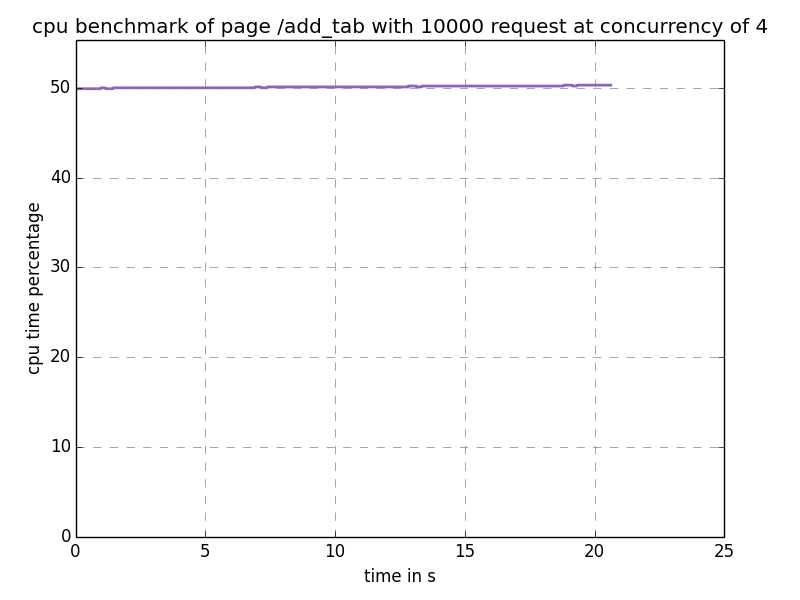
\includegraphics[width=0.5\linewidth]{img/add_tab.cpu.png}
		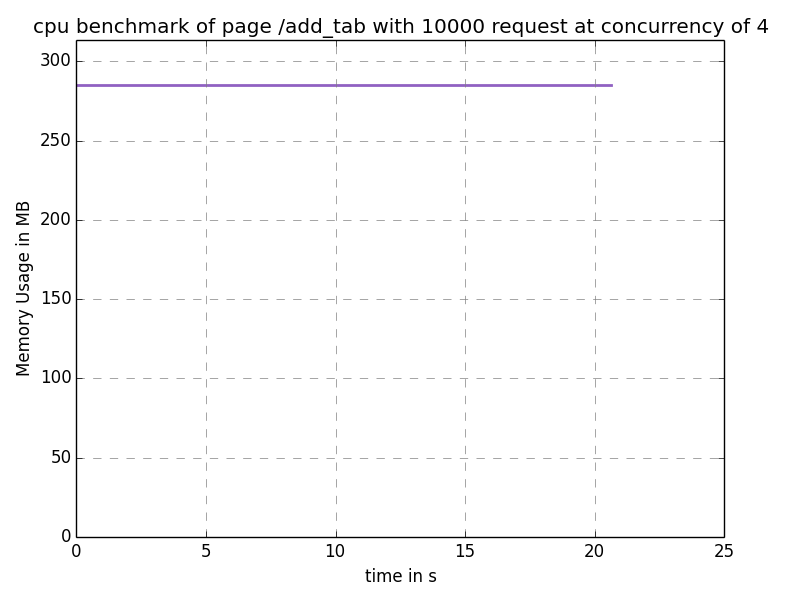
\includegraphics[width=0.5\linewidth]{img/add_tab.mem.png}
		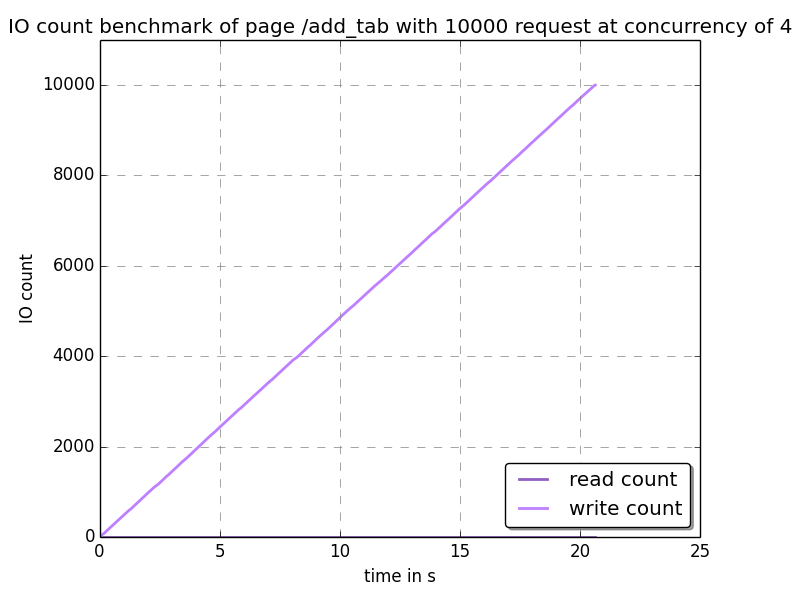
\includegraphics[width=0.5\linewidth]{img/add_tab.io-count.png}
		\caption{Test result of \textbf{add\_tab} API}
	\end{figure}
  \subsection{Converge}
    The converge ratio reached 90\%.
    For more details please refer to appendix converge sheet.

    The code that are not converged is mainly exception handle phase.
    But for each kind of exception handle, at least one case is designed to test it.
    For example, all most all APIs are login required,
    but only one test case that try to logout while not logged in is designed.
    For one kind of exception handle procedure is the same, but may occur in many situation.
    Designing duplicate test cases for each API doesn't means a lot but cause plenty of time.

    For others, they are designed for further widening usage that not implement yet.
    Such as more configurable fetcher, user defined color theme and so on.
